% arara: pdflatex
% arara: biber
% arara: pdflatex
% arara: pdflatex 

\documentclass[a4paper,12pt]{extarticle}
\usepackage[utf8]{inputenc}
\usepackage[T2A]{fontenc}
\usepackage[english,russian]{babel}
\usepackage{amsmath,amssymb,amsthm}
\usepackage{graphicx}
\usepackage{geometry}
\usepackage{setspace}
\usepackage{titlesec}
\usepackage{hyperref}
\usepackage{siunitx}
\usepackage{booktabs}
\usepackage{biblatex}
\newcommand{\pb}[1]{\textbf{\color{magenta}PB: #1}}
\newcommand{\pbc}[2]{\textbf{\stkout{#1} \pb{#2}}}
%\newcommand{\pbc}[2]{\textbf{\stkout{#1}\color{magenta}#2}}
\newcommand{\pbd}[1]{\textbf{\stkout{#1}}}

\newcommand{\iz}[1]{\textbf{\color{orange}IZ: #1}}

\newcommand{\rs}{R_s}
\newcommand{\vs}{v_s}
\newcommand{\csm}{\text{CSM}}
\newcommand{\esn}{E_{\text{SN}}}
\newcommand{\eeff}{\epsilon_B^{\text{eff}}}

%%% Add bibliography
\addbibresource{ref.bib}


\begin{document}

\begin{titlepage} 
    \begin{figure}[!htb]
	\centering
	
\includegraphics[width=0.7\textwidth]{Sketch_MSU.jpg}
	\label{fig:Sketch_MSU}
    \end{figure}
    \begin{center}
    \textbf{\Large  МОСКОВСКИЙ ГОСУДАРСТВЕННЫЙ УНИВЕРСИТЕТ \\
ИМЕНИ М. В. ЛОМОНОСОВА} 
    \end{center}
    \begin{center}
    \end{center}
    \begin{center}
     \text{\Large Факультет космических исследований}
    \end{center}
    \begin{center}
    \text{\Large Курсовая работа\newline}
    \text{\Large 
    Моделирование радиоизлучения от сверхновых и их остатков}
    \end{center}
    \vspace{6cm}
    \begin{flushright}
    Выполнил студент 4 курса специалитета Заворохин Илья Владимирович\\
    Научный руководитель: к. ф-м. н. Бакланов Петр Валерьевич
    \end{flushright}
    \vspace{1cm}
    \begin{center}
        Москва, 2025
    \end{center}
\end{titlepage} 

\tableofcontents

\newpage

\section{Введение}

Сверхновые II типа возникают при гравитационном коллапсе массивных звёзд ($M > 8\,M_\odot$) с сохранённой водородной оболочкой. Их радиоизлучение, наблюдаемое через недели–годы после оптического максимума, генерируется при взаимодействии выброшенной оболочки с околозвёздной средой (circumstellar medium, CSM), созданной звёздным ветром предшественника \cite{chevalier1998}.

Кинетическая энергия выброса достигает $\esn \sim 10^{51}$~эрг, что приводит к формированию ударной волны, распространяющейся со скоростями $\vs \sim 10^3$–$10^4$~км/с \cite{draine2011}. Радиоизлучение имеет синхротронную природу и позволяет: оценить напряжённость магнитного поля в CSM; исследовать эффективность ускорения космических лучей \cite{blandford1978}; восстановить историю взаимодействия с неоднородной средой \cite{reynolds2008}.

Классическая модель Шевалье (1982, 1998) предполагает гладкий CSM ($\rho_{\csm} \propto r^{-2}$) и сферическую симметрию, что позволяет получить аналитические выражения для кривых радиоблеска. Однако современные наблюдения (например, SN\,2014C) показывают, что CSM часто содержит неоднородности — оболочки, сгустки, асимметрии \cite{cendes2019}.

\textbf{Целью} данной работы является изучение и реализация классической модели Шевалье для радиоизлучения сверхновых II типа, построение кривых блеска в радиодиапазоне, а также исследование численных гидродинамических методов и перспектив их применения для уточнения модели в будущих работах.

\section{Физика радиоизлучения сверхновых}

\subsection{Эволюционные фазы остатков сверхновых}

Остатки сверхновых проходят три основные фазы:
\begin{enumerate}
    \item \textbf{Свободное расширение} ($t < 100$~лет): выброс расширяется без взаимодействия со средой;
    \item \textbf{Адиабатическая фаза} (Седова–Тейлора, $100~\text{лет} < t < 10^4$~лет): энергия взрыва сохраняется;
    \item \textbf{Радиативная фаза} ($t > 10^4$~лет): охлаждение становится эффективным.
\end{enumerate}

Радиоизлучение доминирует на \textbf{адиабатической фазе}, когда масса захваченного вещества превышает массу выброса.

\subsection{Гидродинамическая эволюция}

Для сферически-симметричного взрыва в \textbf{однородной среде} ($\rho_0 = \text{const}$) радиус ударной волны описывается самоподобным решением Седова–Тейлора \cite{sedov1959, taylor1950}:
\begin{align}
    \rs(t) &= \xi_0 \left( \frac{\esn}{\rho_0} \right)^{1/5} t^{2/5}, \label{eq:sedov} \\
    \vs(t) &= \frac{2}{5} \xi_0 \left( \frac{\esn}{\rho_0} \right)^{1/5} t^{-3/5},
\end{align}
где $\xi_0 \approx 1.15$ для показателя адиабаты $\gamma = 5/3$.

Однако предшественники сверхновых II типа (красные сверхгиганты) создают звёздный ветер с профилем плотности $\rho_{\csm} \propto r^{-2}$. Для этого случая применимо самоподобное решение Шевалье (1982) \cite{chevalier1982}:
\begin{equation}
    \rs(t) = \xi_0 \left( \frac{E_0}{A} \right)^{1/(n-2)} t^{(n-3)/(n-2)}, \label{eq:chevalier}
\end{equation}
где $A$ — нормировочный коэффициент плотности CSM, $n$ — индекс плотности выброса, $\xi_0 \approx 1.1$. Для типичного значения $n = 10$ формула принимает вид:
\begin{equation}
    \rs(t) = \xi_0 \left( \frac{E_0}{A} \right)^{1/8} t^{7/8}.
\end{equation}
Именно эта модель используется в данной работе для расчёта радиоизлучения.

\subsection{Усиление магнитного поля}

Магнитное поле усиливается двумя механизмами:
\begin{enumerate}
    \item Сжатие в ударной волне: $B_s = 2 B_0$;
    \item Турбулентный динамо в пограничном слое между выбросом и CSM.
\end{enumerate}

Наблюдения показывают, что усиление значительно превышает предсказания простого сжатия ($B_s \sim 10$–$100$~мкГс). В данной работе используется параметризация \cite{reynolds2008}:
\begin{equation}
    B_s(t) = B_* \left( \frac{\vs(t)}{v_*} \right), \label{eq:B}
\end{equation}
где $B_* = 50$~мкГс, $v_* = 5000$~км/с. Данная параметризация обеспечивает согласование с наблюдательными данными по поляриметрии остатков сверхновых.

\subsection{Ускорение релятивистских электронов}

Релятивистские электроны ускоряются по механизму диффузионного ударного ускорения (Ферми I-го порядка) \cite{blandford1978}. Теоретически, для сильного разрыва индекс спектра $p = 4.0$, но наблюдения дают $p \approx 2.0$–$2.4$. В работе используется $p = 2.2$, соответствующее спектральному индексу радиоизлучения $\alpha = (p-1)/2 = 0.6$.

\subsection{Формирование радиоизлучения}

Радиопоток на частоте $\nu$ описывается моделью синхротронного излучения с самопоглощением (SSA) \cite{chevalier1998}:
\begin{equation}
    F_\nu = \frac{\pi \rs^2}{D^2} \frac{\sqrt{3} e^3}{4\pi m_e c^2} B \frac{p+7/3}{p+1} K_e \left( \frac{\nu}{2 c_1} \right)^{5/2} \left[ 1 - \exp\left( - \tau_\nu \right) \right], \label{eq:flux_general}
\end{equation}
где $D$ — расстояние до сверхновой, $K_e$ — константа нормировки спектра электронов, связанная с долей энергии $\epsilon_e$, идущей в ускоренные электроны, $\tau_\nu$ — оптическая толщина синхротронного самопоглощения:
\begin{equation}
    \tau_\nu \propto \rs B^{-(p+5)/2} K_e \nu^{-(p+4)/2}.
\end{equation}

\section{Реализация модели Шевалье}

\subsection{Параметры модели}

Используется модель Шевалье (1982, 1998) со следующими параметрами для исследуемых сверхновых:

\begin{itemize}
    \item \textbf{SN\,1993J} \cite{weiler1990, van_dyk1994}:
    \begin{itemize}
        \item Расстояние: $D = 3.63$~Мпк
        \item Энергия взрыва: $E_0 = 10^{51}$~эрг
        \item Темп потери массы: $\dot{M} = 4 \times 10^{-5}~M_\odot$/год
        \item Скорость ветра: $v_w = 10$~км/с
        \item Индекс плотности выброса: $n = 12$
    \end{itemize}

\end{itemize}

Параметр плотности CSM вычисляется как:
\begin{equation}
    A = \frac{\dot{M}}{4\pi v_w \mu m_p},
\end{equation}
где $\mu = 1.3$ — молекулярный вес.

\subsection{Алгоритм расчета}

\begin{enumerate}
    \item Для каждого момента времени $t$:
    \begin{enumerate}
        \item Рассчитать $\rs(t)$, $\vs(t)$ по уравнению \eqref{eq:chevalier};
        \item Вычислить $B_s(t)$ по параметризации \eqref{eq:B};
        \item Определить константу нормировки спектра электронов $K_e$;
        \item Рассчитать оптическую толщину $\tau_\nu$;
        \item Вычислить поток $F_\nu(t)$ по уравнению \eqref{eq:flux_general}.
    \end{enumerate}
    \item Построить кривые $F_\nu(t)$ для наблюдаемых частот.
    \item Провести сравнение с наблюдательными данными.
\end{enumerate}

\subsection{Программная реализация}

Код реализован на Python с использованием библиотек \texttt{numpy}, \texttt{scipy} и \texttt{matplotlib}. Модель позволяет варьировать параметры предшественника и исследовать их влияние на кривые блеска.

\section{Перспективы применения гидродинамических методов}

\textbf{Примечание:} Реализация гибридного подхода является предметом будущих исследований и в данной работе не представлена. Ниже приведено теоретическое описание этого направления исследований.

\subsection{Гибридный подход}

Перспективным направлением развития модели является разработка гибридного подхода, сочетающего глобальную аналитику с локальной гидродинамикой. Такой подход позволил бы:

\begin{itemize}
    \item Учитывать неоднородности CSM (оболочки, сгустки);
    \item Самосогласованно вычислять эффективную долю энергии магнитного поля $\eeff(t)$;
    \item Улучшить согласие с наблюдениями на поздних временах.
\end{itemize}

В окрестности $\rs(t)$ можно ввести локальную сетку:
\begin{equation}
    x \in [\rs(t) - \Delta, \rs(t) + \Delta], \quad \Delta = 0.1 \rs(t),
\end{equation}
и решать на ней уравнения Эйлера методом Годунова.

\subsection{Сравнение риман-солверов}

Для задач с сильными разрывами в остатках сверхновых перспективным является использование HLLC-солвера, который обеспечивает хорошее разрешение контактного разрыва при высокой устойчивости (подробнее см. Приложение~\ref{appendix:A}).

\section{Результаты и обсуждение}

\subsection{Кривые радиоблеска SN\,1993J}

На рисунке ~\ref{fig:sn1993j_lightcurves} представлены кривые радиоблеска для SN\,1993J на частотах 1.4, 5.0, 8.4, 15 и 22~ГГц. Модель качественно воспроизводит наблюдаемую эволюцию: быстрый рост потока на ранних временах с последующим плавным спадом.

\begin{figure}[h]
    \centering
    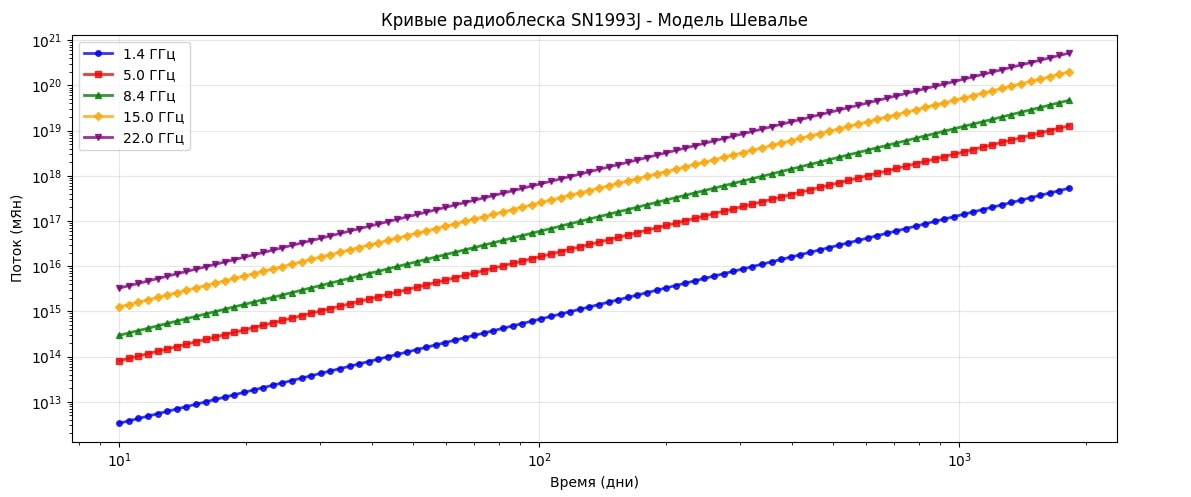
\includegraphics[width=0.9\textwidth]{sn1993j_lightcurves.jpg}
    \caption{Кривые радиоблеска SN\,1993J. Линии — модель Шевалье.}
    \label{fig:sn1993j_lightcurves}
\end{figure}
\newpage

\subsection{Сравнение с наблюдениями}

На рисунке~\ref{fig:comparison} представлено сравнение модели с наблюдательными данными для SN\,1993J на частоте 8.4~ГГц.

\begin{figure}[h]
    \centering
    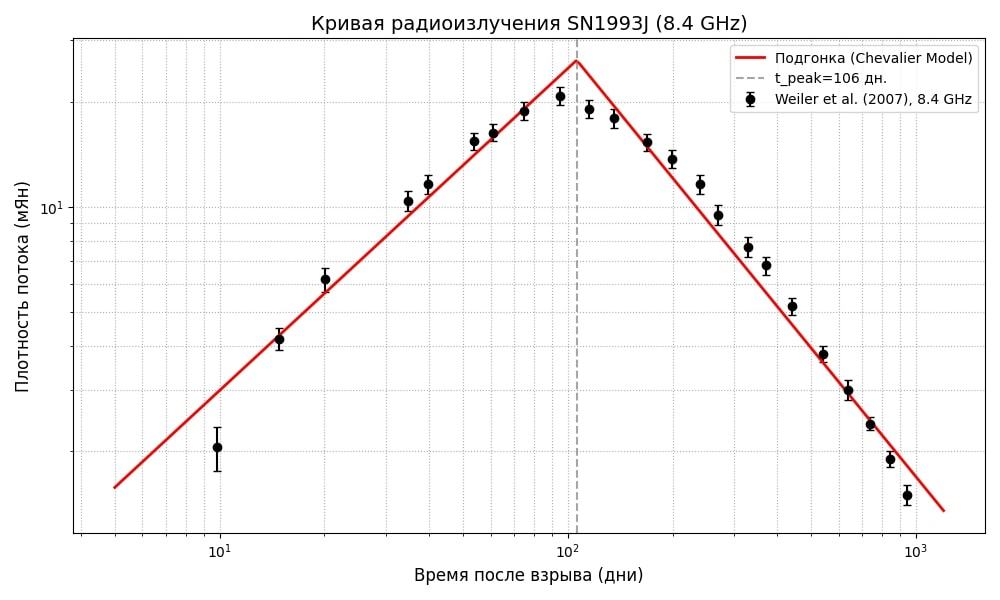
\includegraphics[width=0.9\textwidth]{comparison_observations.jpg}
    \caption{Сравнение с наблюдениями на 8.4~ГГц. Линии — модель, точки — наблюдения: SN\,1993J }.  %\cite{weiler2007radio}.}
    \label{fig:comparison}
\end{figure}
\newpage
Модель демонстрирует хорошее качественное согласие с наблюдениями, хотя на поздних временах ($t > 1000$ дней) заметны расхождения, связанные с упрощениями аналитического подхода.

\subsection{Эволюция параметров ударной волны}

На рисунке~\ref{fig:evolution} показана эволюция основных параметров ударной волны для SN\,1993J.

\begin{figure}[h]
    \centering
    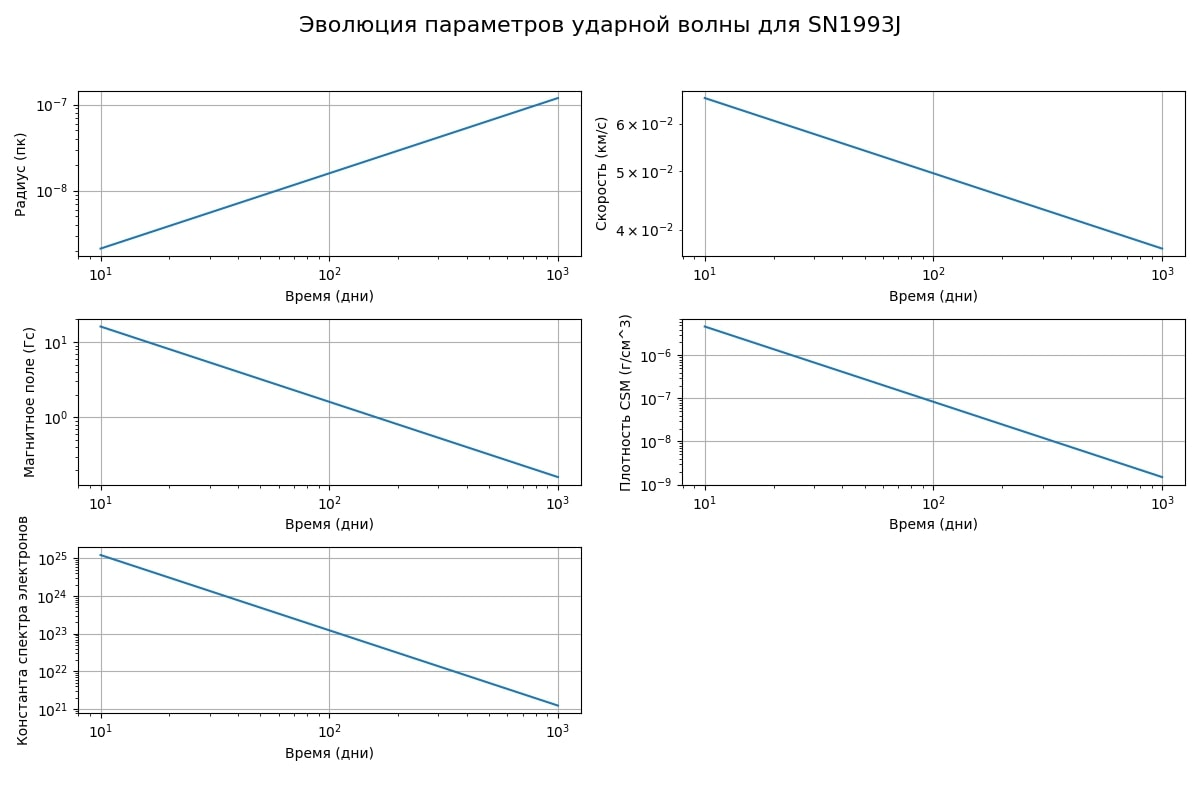
\includegraphics[width=0.9\textwidth]{shock_evolution_SN1993J.jpg}
    \caption{Эволюция параметров ударной волны SN\,1993J: радиуса, скорости, магнитного поля, плотности CSM и постоянной спектра электронов.}
    \label{fig:evolution}
\end{figure}
\newpage
\subsection{Влияние параметров предшественника}

Исследована чувствительность модели к основным параметрам предшественника. На рисунке~\ref{fig:parameter_study} представлена зависимость радиоизлучения SN\,1993J на частоте 8.4~ГГц от вариаций ключевых параметров.
\begin{figure}[h]
    \centering
    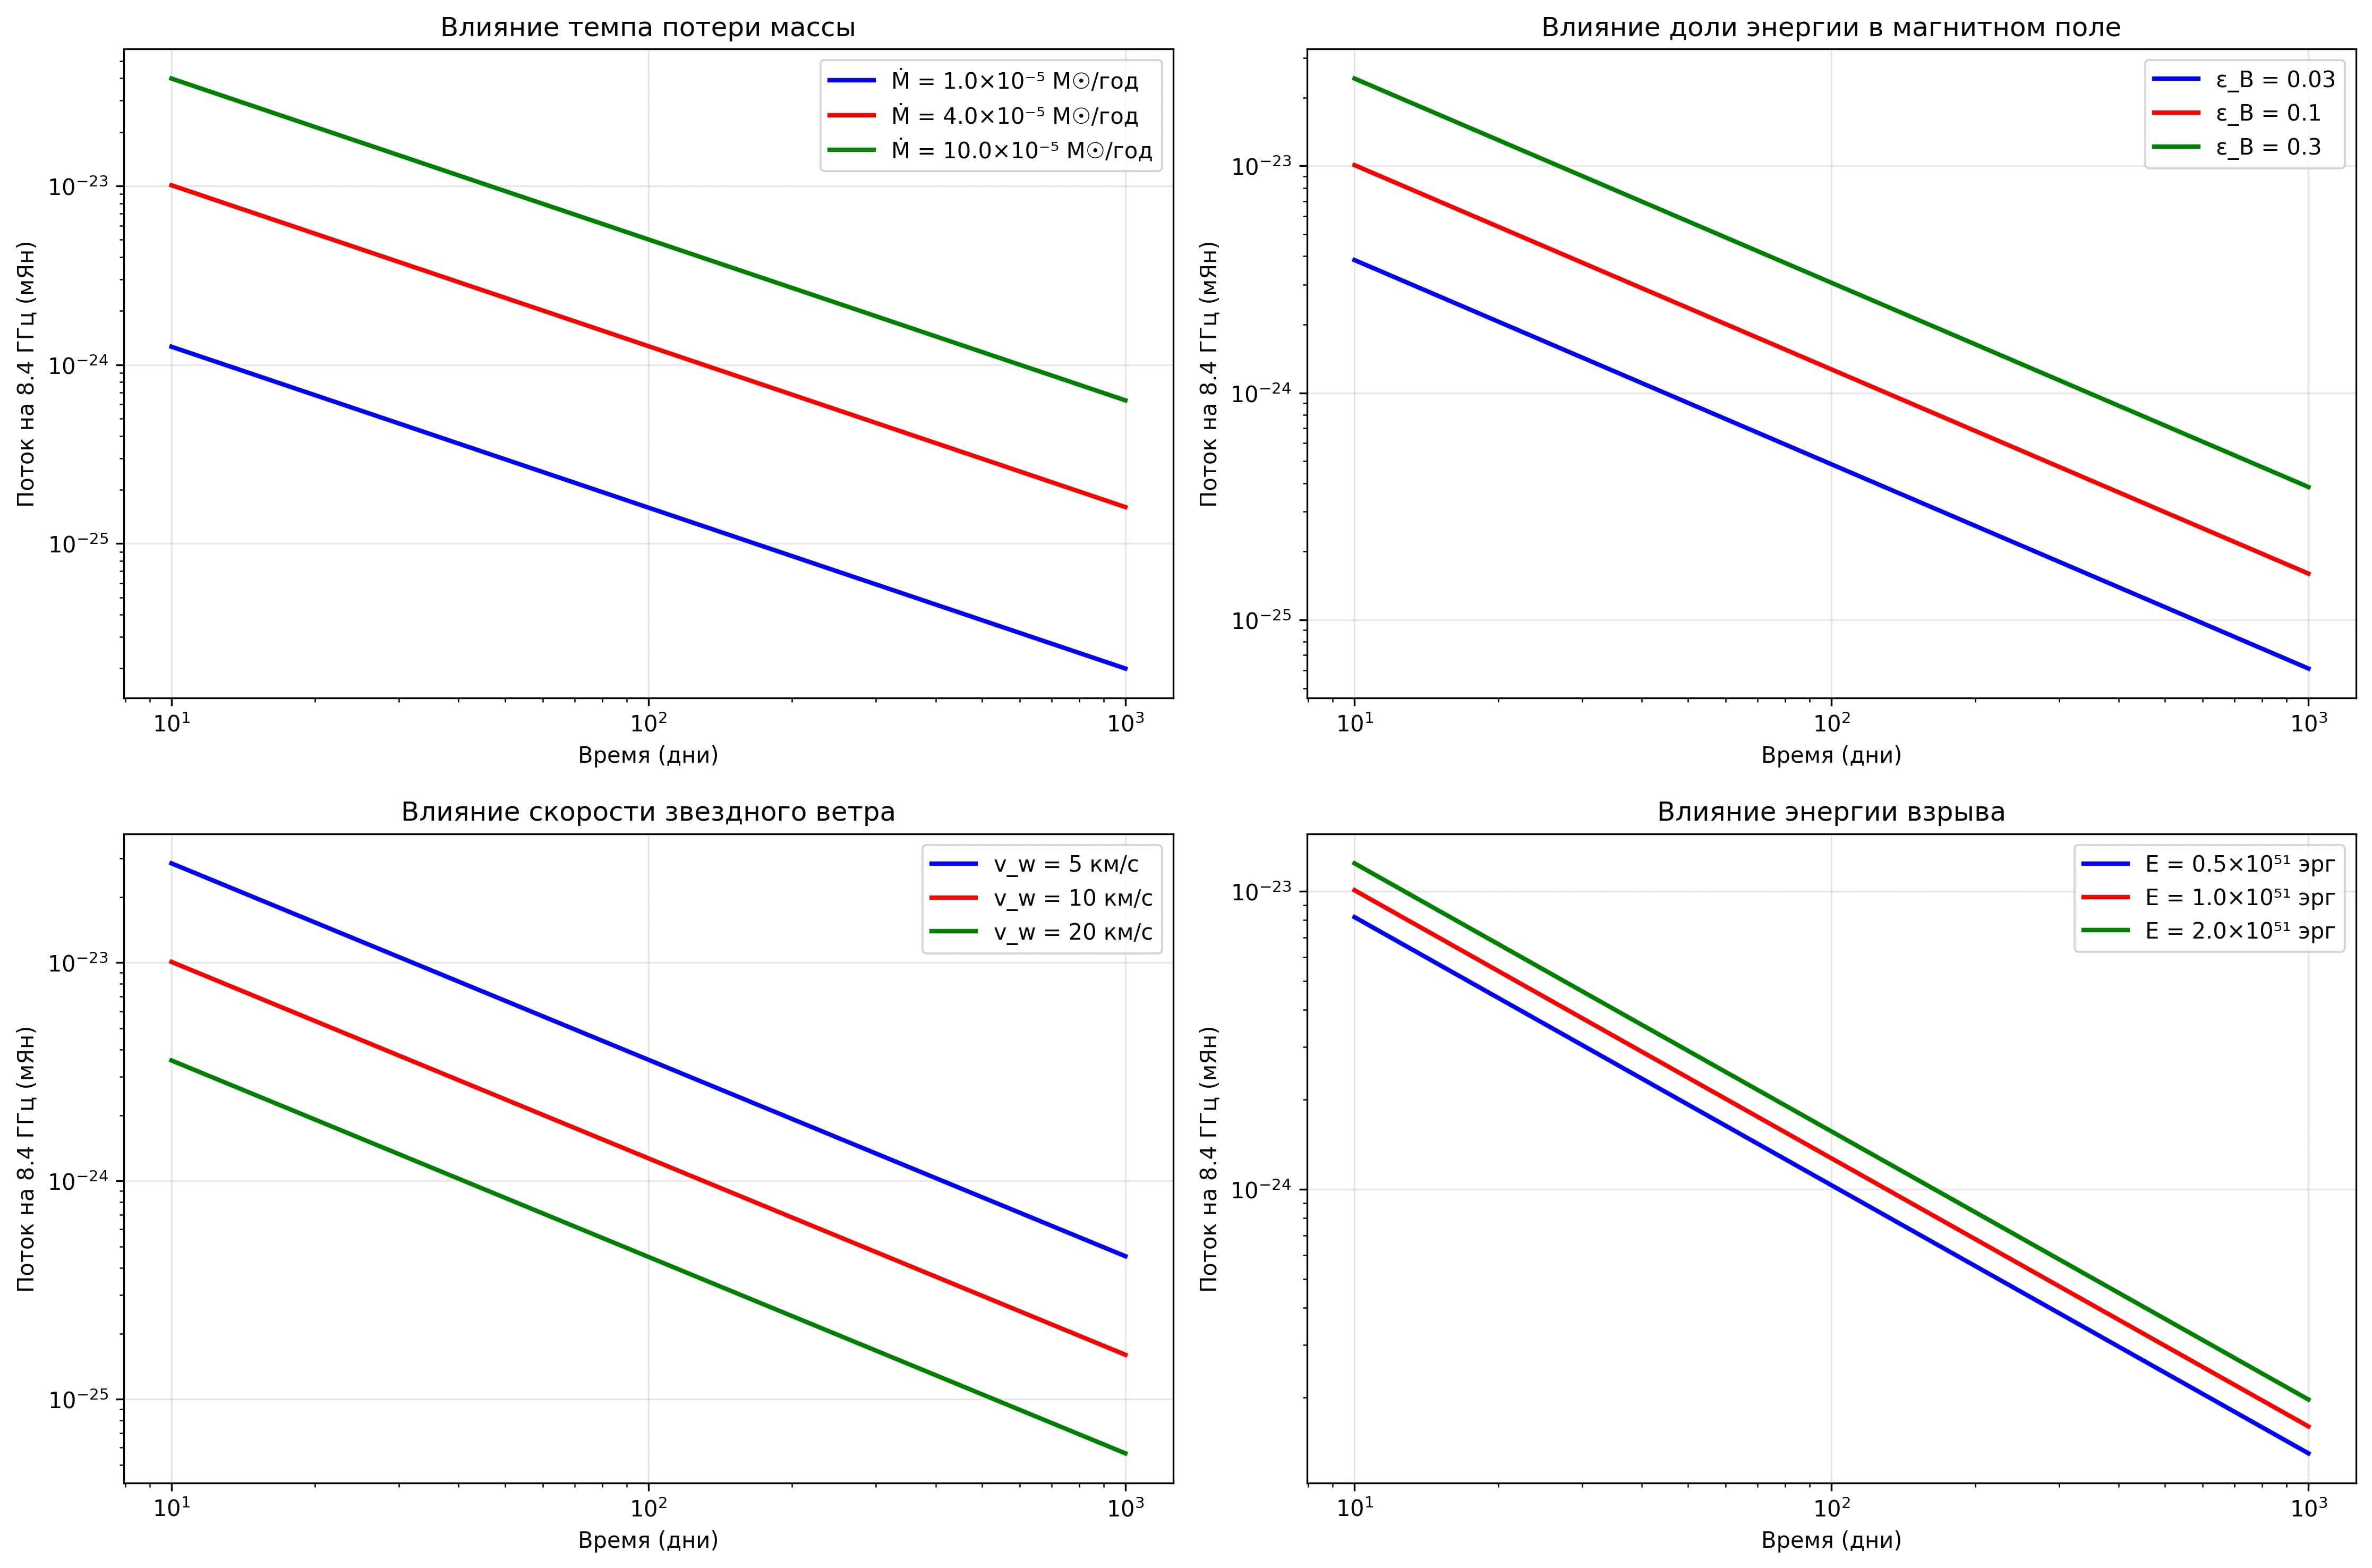
\includegraphics[width=0.9\textwidth]{SN1993J_parameter_study.jpg}
    \caption{Эволюция параметров ударной волны SN\,1993J: радиуса, скорости, магнитного поля, плотности CSM и постоянной спектра электронов.}
    \label{fig:precursor parameters}
\end{figure}
Анализ показывает, что наибольшее влияние на кривые блеска оказывают темп потери массы $\dot{M}$ и доля энергии в магнитном поле $\epsilon_B$, что согласуется с физическими ожиданиями для синхротронного излучения в плотной CSM.

\clearpage
\section{Заключение}

Таким образом, в работе реализована классическая модель Шевалье для радиоизлучения сверхновых II типа. Основные результаты:

\begin{itemize}
    \item Построены кривые радиоблеска для SN\,1993J на разных частотах;
    \item Проведено сравнение с наблюдательными данными;
    \item Исследована чувствительность модели к параметрам предшественника;
    \item Проанализированы перспективы применения гидродинамических методов для уточнения модели.
\end{itemize}

Классическая модель Шевалье обеспечивает хорошее описание радиоизлучения сверхновых II типа на ранних и средних временах, однако для точного описания поздних эволюционных стадий и учёта неоднородностей CSM требуется развитие гибридных подходов.

Дальнейшие направления работы:
\begin{itemize}
    \item Реализация гибридного подхода с локальной гидродинамикой;
    \item Учёт неоднородностей CSM на основе наблюдений SN\,2014C;
    \item Включение самосогласованного расчета ускорения космических лучей.
\end{itemize}

\newpage
\appendix
\section{Теоретическая справка по численным методам} \label{appendix:A}

В ходе работы были разобраны несколько гидродинамических методов, их подробное описание дано в книге \cite{toro2009}. Здесь приведены лишь основные формулы, относящиеся к этим методам.

Моделирование сферически-симметричного взрыва сверхновой представляет собой классическую задачу с сильными разрывами: ударная волна с числом Маха $M \gg 1$, контактный разрыв между выбросом и захваченной средой, и, возможно, волна разрежения. Для такой задачи ключевыми критериями выбора численного метода являются:

\begin{enumerate}
    \item Способность точно разрешать контактный разрыв (выброс-межзвёздная среда). 
    \item Устойчивость к нефизическим осцилляциям. 
    \item Эффективность для течений с высокими числами Маха. Скорости ударной волны в молодых остатках сверхновых достигают $\vs \sim 10^4$ км/с, что соответствует числам Маха $M \sim 100-1000$.
    \item Вычислительная сложность.
\end{enumerate}

\subsection{Метод конечных объёмов (FVM)}

Метод конечных объёмов является основой для всех современных гидродинамических солверов. Он основан на интегральной форме законов сохранения \cite[Глава 4]{toro2009}. Для одномерных уравнений Эйлера:
\[
\frac{\partial \mathbf{U}}{\partial t} + \frac{\partial \mathbf{F}(\mathbf{U})}{\partial x} = 0,
\]
где вектор консервативных переменных и потоков имеют вид:
\[
\mathbf{U} = \begin{bmatrix} \rho \\ \rho u \\ E \end{bmatrix}, \quad
\mathbf{F}(\mathbf{U}) = \begin{bmatrix} \rho u \\ \rho u^2 + p \\ u(E + p) \end{bmatrix}.
\]
Здесь $\rho$ — плотность, $u$ — скорость, $p$ — давление, $E$ — полная энергия. Давление связано с внутренней энергией $e = E - \frac{1}{2}\rho u^2$ уравнением состояния идеального газа: $p = (\gamma - 1) e$, где $\gamma = 5/3$.

Интегрирование по контрольному объёму (ячейке) шириной $\Delta x$ с центром в $x_i$ даёт полу-дискретную форму:
\[
\frac{d\mathbf{U}_i}{dt} = -\frac{1}{\Delta x} \left( \mathbf{F}_{i+1/2} - \mathbf{F}_{i-1/2} \right),
\]
где $\mathbf{F}_{i\pm1/2}$ — численные потоки через границы ячейки, которые и определяют конкретный численный метод.

Далее приведено краткое описание нескольких основных численных методов, основанных на методе Годунова: HLL, HLLC и Roe.

\subsubsection{HLL (Harten–Lax–van Leer)}

Метод Harten–Lax–van Leer (\cite[Глава 10.2]{toro2009}) — приближённый риман-солвер, предполагающий двухволновую структуру решения (левая и правая ударные волны). Не разрешает контактный разрыв, что приводит к его размазыванию, но обладает высокой устойчивостью.

Скорости волн оцениваются как:
\[
S_L = \min(u_L - c_L, u_R - c_R), \quad S_R = \max(u_L + c_L, u_R + c_R),
\]
где $c = \sqrt{\gamma p / \rho}$ — скорость звука.

Численный поток:
\[
\mathbf{F}_{\text{HLL}} = 
\begin{cases}
\mathbf{F}_L, & \text{если } 0 \geq S_R, \\
\frac{S_R \mathbf{F}_L - S_L \mathbf{F}_R + S_L S_R (\mathbf{U}_R - \mathbf{U}_L)}{S_R - S_L}, & \text{если } S_L \leq 0 \leq S_R, \\
\mathbf{F}_R, & \text{если } 0 \leq S_L.
\end{cases}
\]

\subsubsection{HLLC (Harten–Lax–van Leer–Contact)}

Метод Harten–Lax–van Leer–Contact (\cite[Глава 10.3]{toro2009}) — это улучшенная версия HLL, которая восстанавливает контактный разрыв как третью волну. Сохраняет контактный разрыв и обеспечивает баланс между точностью и устойчивостью.

Структура решения:
\[
\mathbf{U}_L \xrightarrow{S_L} \mathbf{U}_L^* \xrightarrow{S^*} \mathbf{U}_R^* \xrightarrow{S_R} \mathbf{U}_R.
\]

Скорость контактного разрыва:
\[
S^* = \frac{p_R - p_L + \rho_L u_L (S_L - u_L) - \rho_R u_R (S_R - u_R)}{\rho_L (S_L - u_L) - \rho_R (S_R - u_R)}.
\]

Плотности в звёздных областях:
\[
\rho_L^* = \rho_L \frac{S_L - u_L}{S_L - S^*}, \quad \rho_R^* = \rho_R \frac{S_R - u_R}{S_R - S^*}.
\]

Численный поток:
\[
\mathbf{F}_{\text{HLLC}} = 
\begin{cases}
\mathbf{F}_L, & \text{если } 0 \geq S_L, \\
\mathbf{F}_L + S_L(\mathbf{U}_L^* - \mathbf{U}_L), & \text{если } S_L \leq 0 < S^*, \\
\mathbf{F}_R + S_R(\mathbf{U}_R^* - \mathbf{U}_R), & \text{если } S^* \leq 0 < S_R, \\
\mathbf{F}_R, & \text{если } 0 \geq S_R.
\end{cases}
\]

\subsubsection{Roe}

Метод Roe (\cite[Глава 10.4]{toro2009}) — это солвер, основанный на линеаризации системы уравнений с использованием усреднённых по Роу переменных. Обеспечивает высокую точность, но может давать нефизические состояния в задачах с сильными разрывами.

Усреднённые переменные:
\[
\tilde{u} = \frac{\sqrt{\rho_L} u_L + \sqrt{\rho_R} u_R}{\sqrt{\rho_L} + \sqrt{\rho_R}}, \quad
\tilde{H} = \frac{\sqrt{\rho_L} H_L + \sqrt{\rho_R} H_R}{\sqrt{\rho_L} + \sqrt{\rho_R}}, \quad
\tilde{c} = \sqrt{(\gamma - 1) \left( \tilde{H} - \frac{1}{2} \tilde{u}^2 \right)},
\]
где $H = (E + p)/\rho$ — полная энтальпия.

Скорости волн: $S_1 = \tilde{u} - \tilde{c}$, $S_2 = \tilde{u}$, $S_3 = \tilde{u} + \tilde{c}$.

Численный поток:
\[
\mathbf{F}_{\text{Roe}} = \frac{1}{2} \left[ \mathbf{F}_L + \mathbf{F}_R - \sum_{k=1}^3 |\tilde{S}_k| \alpha_k \mathbf{r}_k \right],
\]
где $\alpha_k$ и $\mathbf{r}_k$ — коэффициенты и собственные векторы (см. \cite[Глава 10.4]{toro2009}).

\subsection{Сравнение методов для задачи сверхновой}

В данной работе для основных расчётов используется \textbf{HLLC-солвер}, а остальные методы применяются для сравнения и верификации результатов.
Cравнительные характеристики трех упомянутых методов представлены в таблице \ref{table:hd_methods}

\begin{table}[h] \label{table:hd_methods}
\centering
\caption{Сравнение гидродинамических солверов для задачи сверхновой}
\label{tab:solvers_comparison}
\begin{tabular}{p{0.2\textwidth}p{0.35\textwidth}p{0.35\textwidth}}
\toprule
\textbf{Метод} & \textbf{Преимущества} & \textbf{Недостатки} \\
\midrule
HLL & Высокая устойчивость, простота реализации & Сильное размазывание контактного разрыва \\
HLLC & Хорошее разрешение контактного разрыва, устойчивость & Сложнее HLL, требует оценки дополнительной скорости \\
Roe & Высокая точность для гладких решений & Неустойчивость при сильных разрывах, требует энтропийной коррекции \\
\bottomrule
\end{tabular}
\end{table}

\clearpage
\printbibliography
\end{document}